\documentclass[a4paper,bcor=0mm,9pt,parskip=full,twoside]{tubsartcl}
\usepackage[utf8]{inputenc}

\usepackage[balancingshow]{multicol}

\usepackage{lipsum}

\begin{document}

% \begin{gaussbox}[bgcolor=tubsOrange20,fgcolor=tuOrange]{1}{1}{6}{8}
\headline{\color{tuOrange}Headline Sans 45pt.\\
Dunt acilluptat Putat-\\
quamacone sit}
\vspace*{2.5cm}
\setlength\postmulticols{0mm}
\begin{minipage}{\textwidth}
\begin{multicols}{2}
\lipsum[2]\par~\par\columnbreak
\lipsum[4]\par
\end{multicols}
\end{minipage}
\vspace*{0.5cm}
\begin{multicols*}{2}
\bfseries\sffamily Diagrammüberschrif in Nexus Sans Bold\par
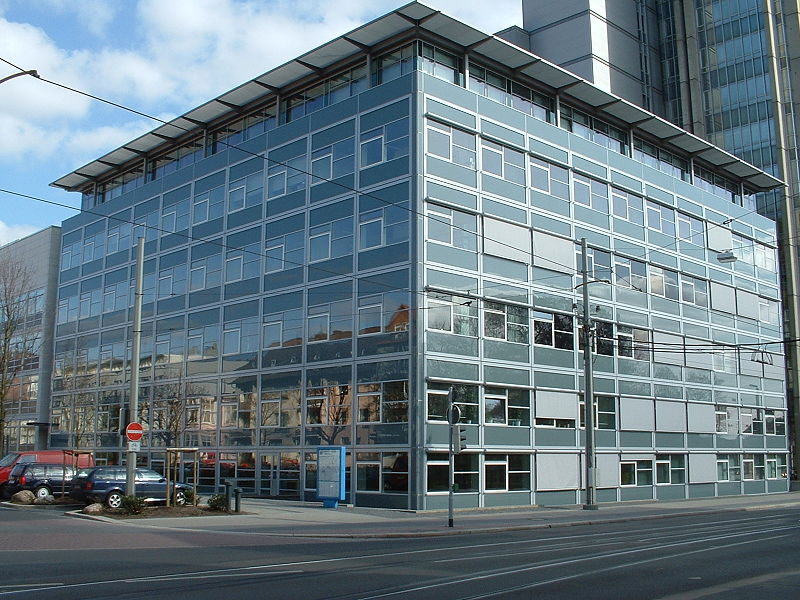
\includegraphics[width=\linewidth]{infozentrum}
\end{multicols*}
\clearpage

\begin{gaussbox}[bgcolor=tubsGray20]{1}{1}{4}{2}
\end{gaussbox}
\begin{gaussbox}[bgcolor=tubsGray20]{5}{1}{2}{1}
\end{gaussbox}
\begin{gaussbox}[bgcolor=tubsGray20]{5}{2}{2}{1}
\end{gaussbox}
\begin{gaussbox}[bgcolor=tuOrangeLight]{1}{3}{6}{6}
\twocolumn[]%
\lipsum[2]\par
\lipsum[2]\par
\end{gaussbox}
\clearpage

\begin{gaussbox}{1}{1}{5}{1}
{\LARGE\sffamily\bfseries Atueriliquat volore feui eui bla
aliquissit atie vulla feum vent
adipit wis acipsus cipit, si.\par}
\end{gaussbox}
\begin{gaussbox}{2}{2}{5}{1}
\usekomafont{institute}\mdseries
Verostrud eugiamet vel dolor ilismolummy nosto conse mod tie
faccum vullan hendit landipisim veraessim vel ullutim irilluptat volor
sequamc onsectet, qui eu facilit alit, vel utpat lore ming eratie dolor
inci bla feuguero odionsed eniamco veliquat lam Dignit atetum verit
ex erit velisci llandigna famur.
\end{gaussbox}
\begin{gaussbox}[bgcolor=tuGray20]{1}{3}{5}{6}
\lipsum[2]\par
\lipsum[2]\par
\end{gaussbox}
\clearpage~\clearpage

\begin{gaussbox}[]{1}{1}{1}{1}
\scriptsize\bfseries\raggedright
Ecte min utpat verilit
luptat adigna alisi blaor
sum dolore feum ipisci-
lisi et aliquis eu faccum-
san vel utet lore do-
lendrem iuscil ut
illandreet et alit illan ul-
putpat amconum deliqui
sciduipsum acincipisi.
Am, conulla faccumsan
henibh et am zzriure
min henis nit wisi.
\end{gaussbox}
\begin{gaussbox}[bgcolor=tubsGray20]{2}{1}{3}{1}
\end{gaussbox}
\begin{gaussbox}[bgcolor=tubsGray20]{5}{1}{2}{1}
\end{gaussbox}
\begin{gaussbox}[bgcolor=tubsGray20]{2}{2}{5}{2}
\end{gaussbox}
\begin{gaussbox}{2}{4}{5}{2}
\raggedright\sffamily
\lipsum[1]
\end{gaussbox}
\clearpage


\end{document}
